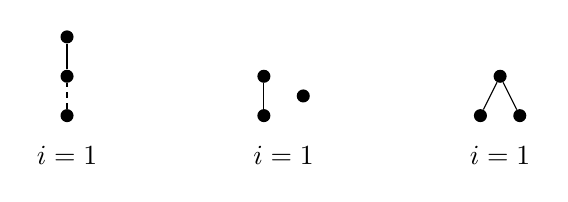
\begin{tikzpicture}
  \uncover<1->{
    \node[circle,fill=black,scale=0.5] (A1) at (0, 0) {};
    \node[circle,fill=black,scale=0.5] (A2) at (0, 0.5) {};
    \node[circle,fill=black,scale=0.5] (A3) at (0, 1) {};

    \draw[dash pattern=on 2pt off 2pt] (A1) -- (A2) node {};
    \draw (A2) -- (A3) node {};
    \node (AL) at (0, -0.5) {$i = 1$};
  }

  \uncover<2->{
    \node[circle,fill=black,scale=0.5] (B1) at (2.5 + 0, 0) {};
    \node[circle,fill=black,scale=0.5] (B2) at (2.5 + 0, 0.5) {};
    \node[circle,fill=black,scale=0.5] (B3) at (2.5 + 0.5, 0.25) {};

    \draw (B1) -- (B2) node {};
    \node (BL) at (2.5 + 0.25, -0.5) {$i = 1$};
  }

  \uncover<3->{
    \node[circle,fill=black,scale=0.5] (C1) at (5 + 0.5, 0.5) {};
    \node[circle,fill=black,scale=0.5] (C2) at (5 + 0.25, 0) {};
    \node[circle,fill=black,scale=0.5] (C3) at (5 + 0.75, 0) {};

    \draw (C1) -- (C2) node {};
    \draw (C1) -- (C3) node {};
    \node (CL) at (5 + 0.5, -0.5) {$i = 1$};
  }
\end{tikzpicture}